
%(BEGIN_QUESTION)
% Copyright 2007, Tony R. Kuphaldt, released under the Creative Commons Attribution License (v 1.0)
% This means you may do almost anything with this work of mine, so long as you give me proper credit

Shown here is the schematic diagram of a full ``PID'' analog electronic controller.  Although it lacks the features of output and setpoint tracking, it does possess all three control terms: Proportional, Integral, and Derivative.

$$\includegraphics[width=15.5cm]{i01635x01.eps}$$

Based on your analysis of this circuit, answer the following questions:

\medskip 
\item{}At what test point would you measure the controller's derivative term signal?
\vskip 5pt
\item{}At what test point would you measure the controller's error signal?
\vskip 5pt
\item{}At what test point would you measure the controller's setpoint signal?
\vskip 5pt
\item{}Which potentiometer adjusts the integral constant ($\tau_i$)?
\vskip 5pt
\item{}Which potentiometer adjusts the derivative constant ($\tau_d$)?
\vskip 5pt
\item{}Which capacitor is used to calculate the integral term?
\vskip 5pt
\item{}Will adjustment of the proportional constant affect either the integral or derivative responses?
\end{itemize} 

\vfil 

\underbar{file i01635}
\eject
%(END_QUESTION)





%(BEGIN_ANSWER)

This is a graded question -- no answers or hints given!

%(END_ANSWER)





%(BEGIN_NOTES)

In order to answer these questions, you must first properly identify the function of each circuit ``module'' in this controller.

\vskip 10pt

{\it At what test point would you measure the controller's derivative term signal?}

At {\bf TP7}, right at the output of the lowest op-amp where derivative is calculated.
 
\vskip 10pt

{\it At what test point would you measure the controller's error signal?}

At the output of the differential amplifier, at {\bf TP3}.
 
\vskip 10pt

{\it At what test point would you measure the controller's setpoint signal?}

At the output of the setpoint potentiometer buffer, {\bf TP2}.
 
\vskip 10pt

{\it Which potentiometer adjusts the integral constant ($\tau_i$)?}

Potentiometer {\bf R3} at the input of the op-amp.
 
\vskip 10pt

{\it Which potentiometer adjusts the derivative constant ($\tau_d$)?}

Potentiometer {\bf R4} in the feedback loop of the op-amp.
 
\vskip 10pt

{\it Which capacitor is used to calculate the integral term?}

Capacitor {\bf C1}, which is in series with potentiometer $R_3$.
 
\vskip 10pt

{\it Will adjustment of the proportional constant affect either the integral or derivative responses?}

No, because the output of the inverting amplifier (where potentiometer $R_2$ sets the gain) does not connect to the inputs of either the integral or derivative sections of the controller circuit.  Instead, the output of the proportional section is merely added to the integral and derivative term signals (along with the bias signal).  This makes the P, I, and D constants independent of one another.
 
%INDEX% Control, proportional + integral + derivative: analog electronic controller

%(END_NOTES)


